\chapter{装置} \label{equipment}
\section{探索装置の概要}
今回の実験に用いた探索装置の概略図及び座標軸を図4.1に、$Y$方向から見た図を図4.2に示す。

\begin{figure}[H]
    \begin{minipage}[b]{0.47\linewidth}
        \centering
        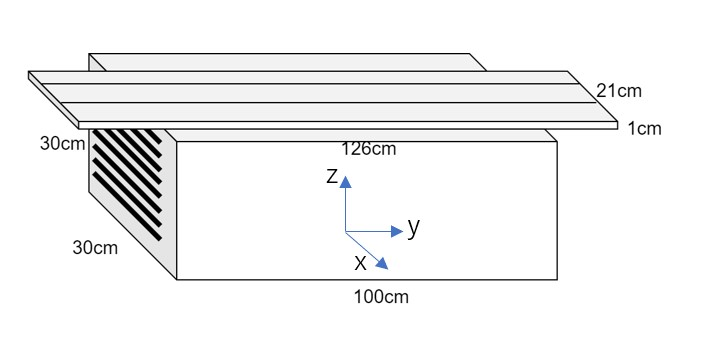
\includegraphics[height=3.5cm]{img/equipment.jpg}
        \caption{探索装置の概略図}
    \end{minipage}
    \begin{minipage}[b]{0.47\linewidth}
        \centering
        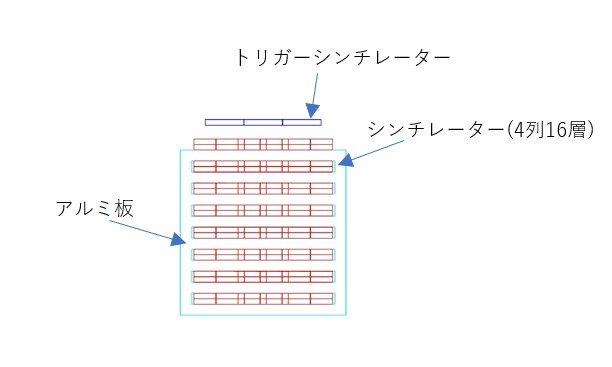
\includegraphics[height=4.3cm]{img/equipment_y.jpg}
        \caption{Y方向から見た装置}
    \end{minipage}
\end{figure}

実験装置は、2cmのアルミ板を2cm間隔で8段積み上げている。
アルミ板の各層には、通過粒子の$xy$平面での座標を特定するためプラスチックシンチレータを逆側に7度ずつ傾けたものを2層ずつ配置している。
この2次元飛跡検出器を$z$方向に8段重ねることで3次元飛跡検出器とし反応の探索を行った。
プラスチックシンチレータからの光は波長変換ファイバーによって伝えられ、光検出器であるMPPCを用い検出しEASIROC MODULEを用いてデジタル信号として読み出された。
また検出装置に入射する$\mu$粒子を検出装置の上方から入射し検出器を通過するものに制限するため、装置上部にプラスチックシンチレータを3枚配置しトリガーシンチレータとして用いた。

\section{装置詳細}
\subsection{プラスチックシンチレータ}
反応の探索に用いたプラスチックシンチレータの大きさは厚さ1cm、長さ75cm、幅4cmである。
プラスチックシンチレータは荷電粒子が通過すると電子が励起し、基底状態に戻るときにシンチレーション光と呼ばれる光を発する荷電粒子検出器である。
このプラスチックシンチレータを4枚を2層ずつ8段配置し、計64枚使用している。

\subsection{波長変換ファイバー}
波長変換ファイバーはプラスチックシンチレータからの光を吸収し、光検出器の感度が良い波長(400~500nm)に変換する。
直径1.2mmのものを使用し、装置片側の基盤に取り付けた光検出器にプラスチックシンチレータからの光を導いた。

\begin{figure}[H]
    \centering
    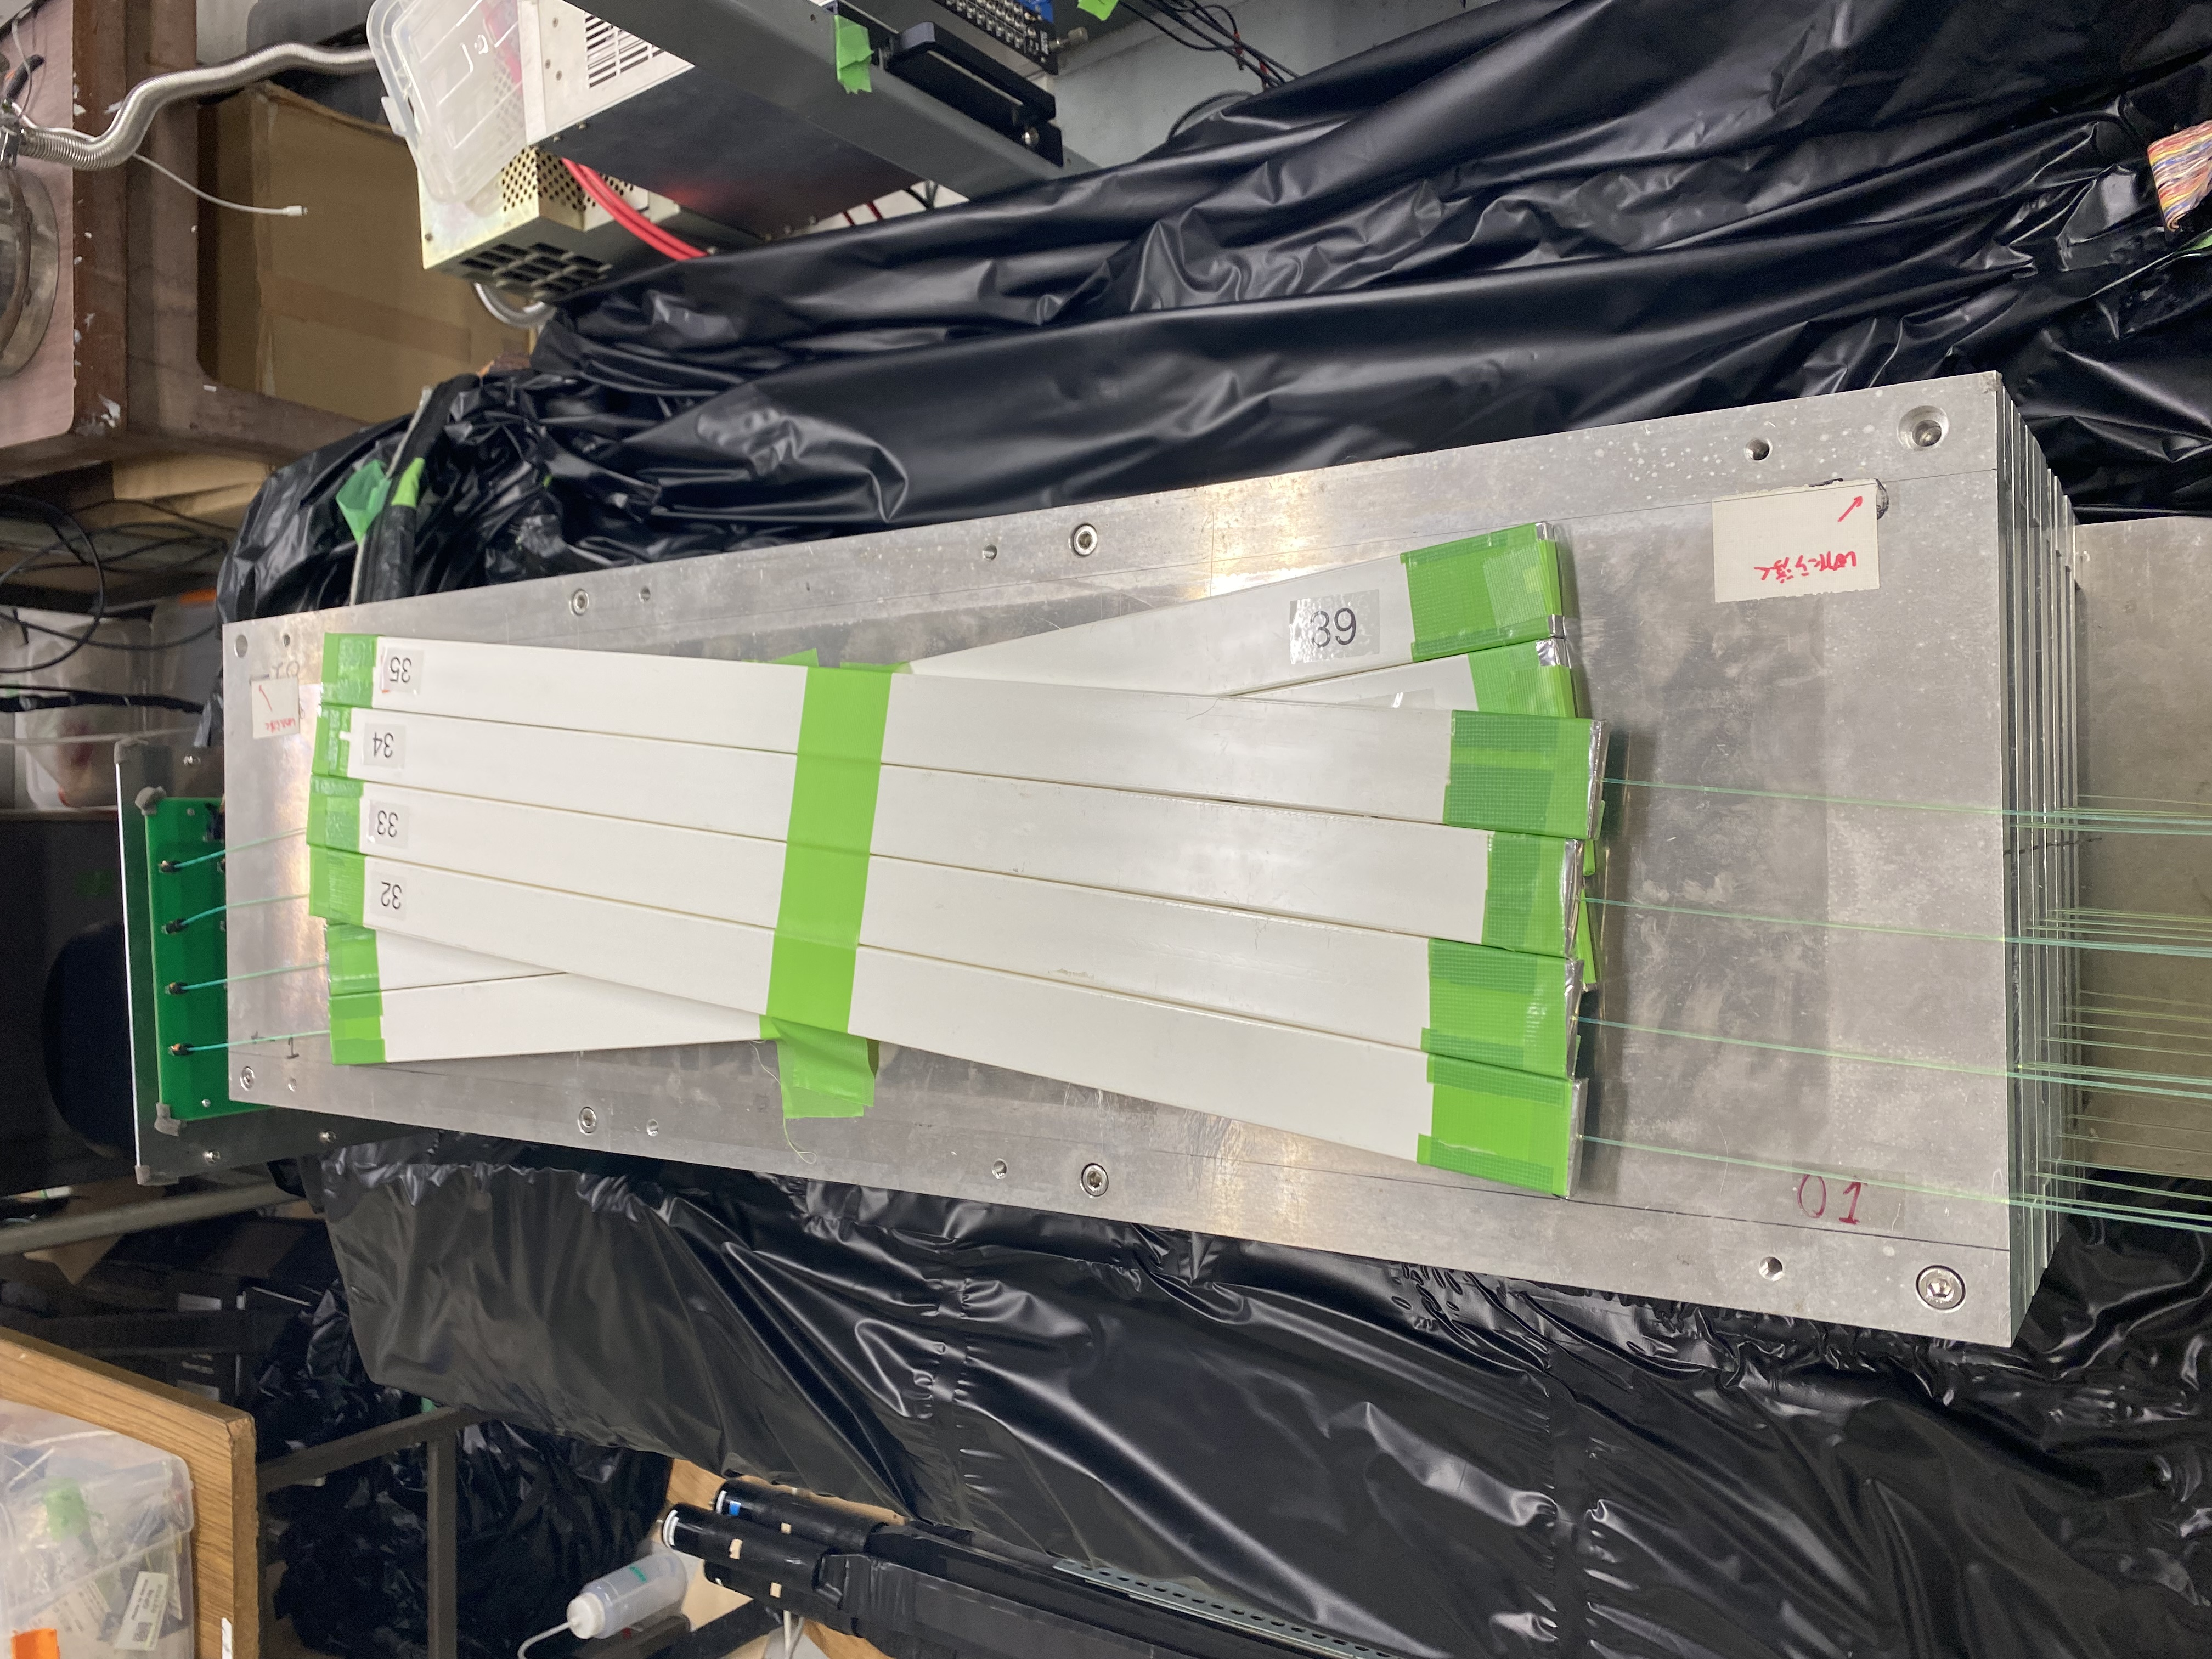
\includegraphics[height=5cm]{img/Scinti.jpeg}
    \caption{プラスチックシンチレータと光ファイバー}
\end{figure}

\subsection{MPPC}
光検出器として、MPPC(Multi Pixel Photon Counter)を用いた。
MPPCは受光面が複数のピクセルからなるフォトンカウンティングデバイスである。各ピクセルは高い増幅率を持つ半導体光検出器である。
各ピクセルにおいて降伏電圧以上で光電子をアバランシェ増幅し、ピクセル内に発生した光電子数によらず同じ波高を出力する。
さらに複数のピクセルで発生した波高は重ね合わせて出力される。
この波高から検出した光電子数を見積もることができる。
このMPPC64個を基板に取り付け、ゴミコネクタを用いてプラスチックシンチレータの片側から出ている波長変換ファイバーと接続した。

\begin{figure}[H]
    \begin{minipage}[b]{0.47\linewidth}
        \centering
        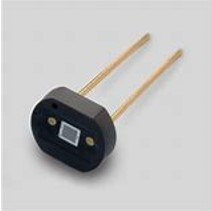
\includegraphics[height=4.5cm]{img/1_mppc.jpg}
        \caption{MPPC}
    \end{minipage}
    \begin{minipage}[b]{0.47\linewidth}
        \centering
        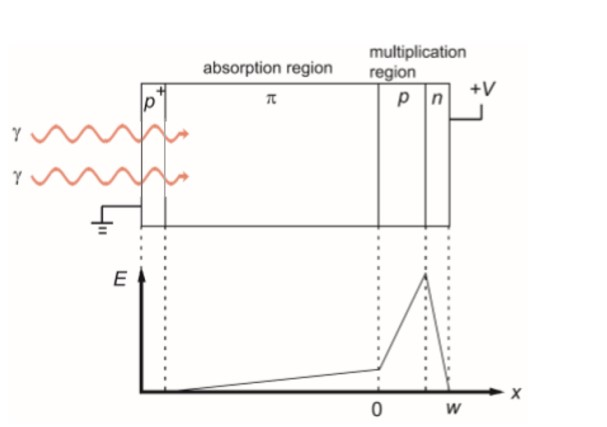
\includegraphics[height=4.5cm]{img/avalanche.jpg}
        \caption{アバランシェ増幅}
    \end{minipage}
\end{figure}

\subsection{EASIROC}
MPPCからの信号の読み出しにEASIROC(Extended Analogue Silicon PM Integrated Read Out Chip)を用いた。
最大64chのMPPCへの電圧の印加や同時読み出しが可能である。

\begin{figure}[H]
    \centering
    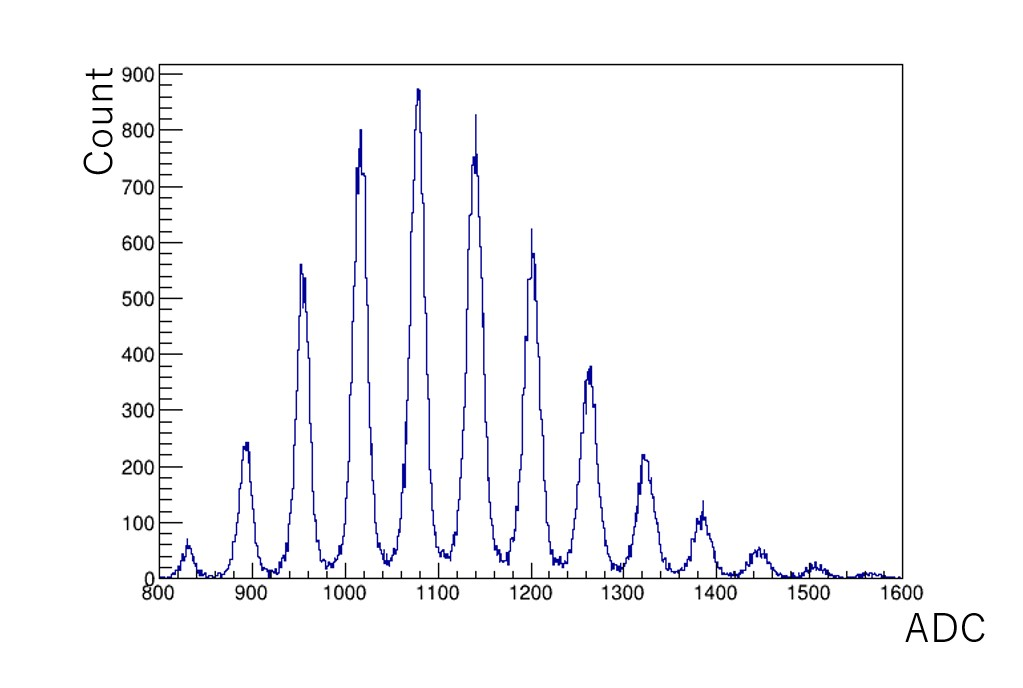
\includegraphics[height=5cm]{img/mppc_easiroc.jpg}
    \caption{EASIROCを用いて読み出したMPPCの信号}
\end{figure}

Amp、Shaper、Discriminator が内蔵されており、光電子数の情報をADC(Analog to Digital Converter)で、時間情報を TDC(Time to Digital Converter) で取得できる。
MPPC にかける電圧はEASIROCによる全チャンネル一律の値の$V_0$ と、Input DACという値を入力することでコントロールした。
Input DACによりコントロールする電圧($V_i$)は、
\begin{equation}
    V_i = -0.0195(InputDAC) + 9.4479
\end{equation}
である。
また、$V_i$と$V_0$とBias Voltage($V$)の関係は
\begin{equation}
    V = V_0 - V_i
\end{equation}
である。
InputDACを調整することで各MPPCへのBias Voltageを調整した。

\subsection{トリガーシンチレータ}
装置のすぐ上に、トリガーシンチレータとして厚さ1cm、長さ126cm、幅7cmのプラスチックシンチレータを3枚設置した。
\begin{figure}[H]
    \centering
    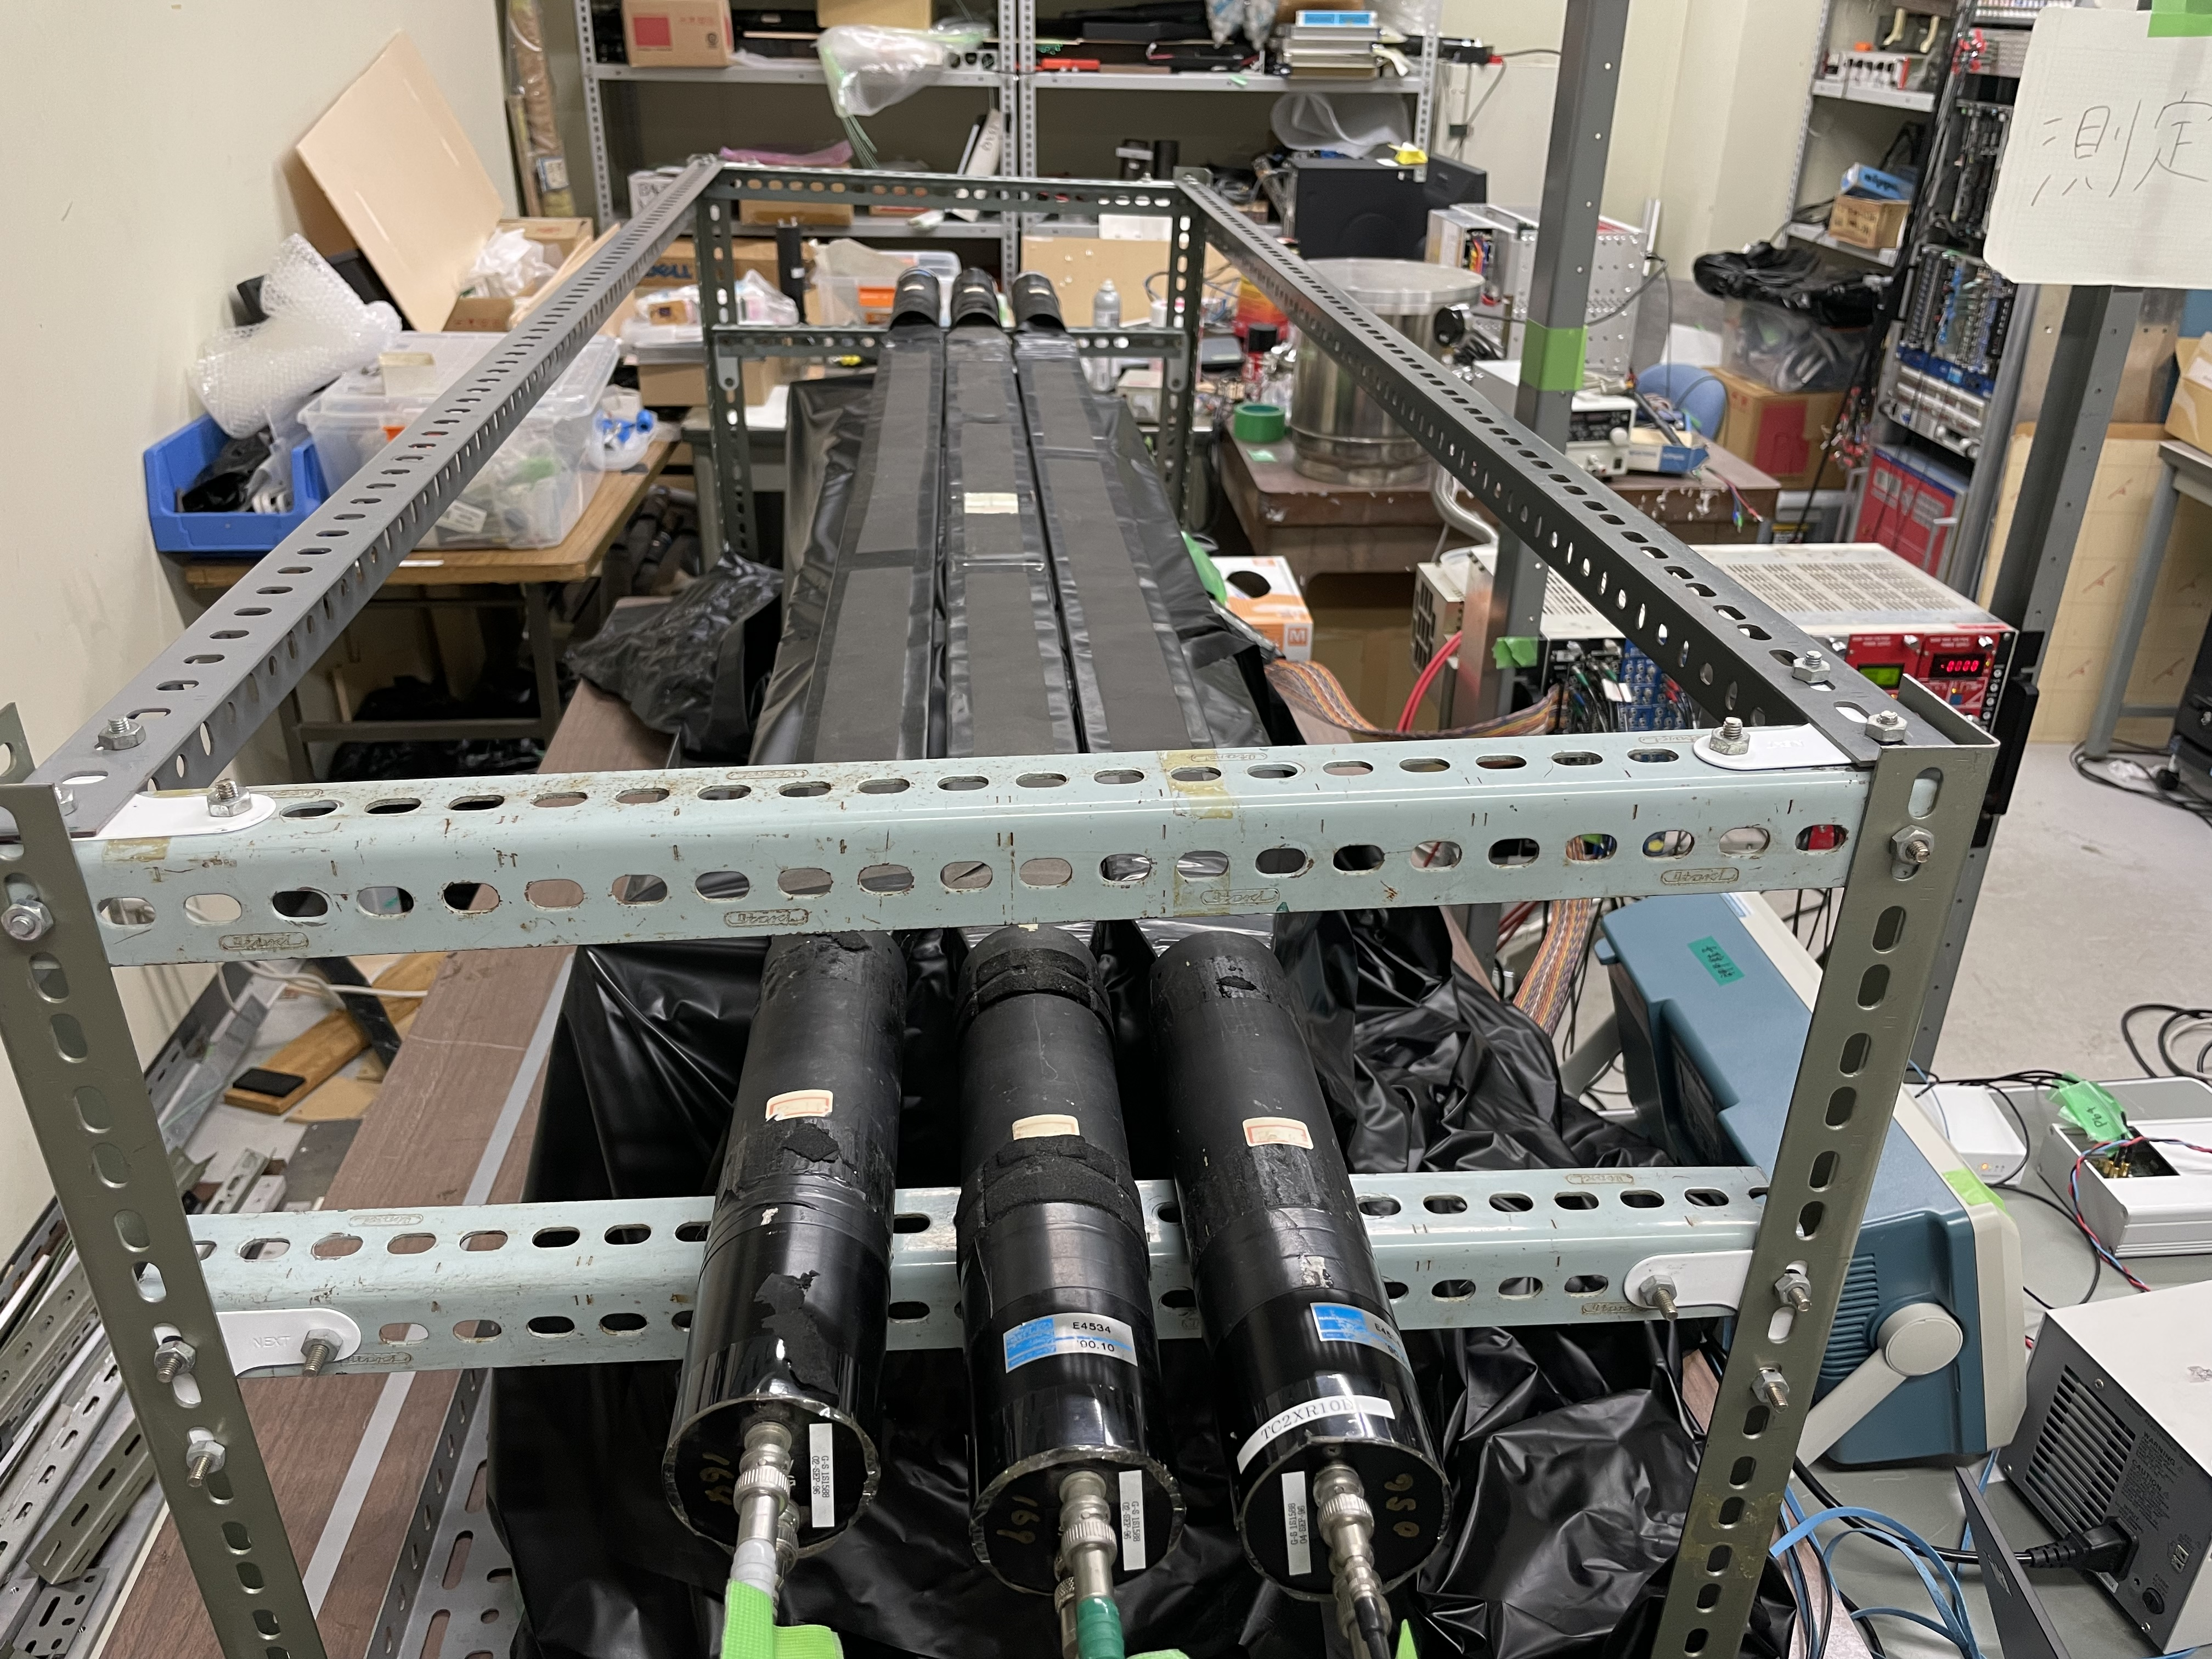
\includegraphics[height=5cm]{img/Trigger.jpeg}
    \caption{トリガーシンチレータの配置}
\end{figure}

\subsection{アルミ板}
厚さ2cm、長さ100cm、幅30cmのアルミの板を2cm間隔で8段積み上げた。
プラスチックシンチレータの間にアルミの板を用いたのは、装置の質量を稼ぎ反応を起こしやすくするためである。

\section{データ取得のセットアップ}
図4.8は今回の実験におけるデータ取得のセットアップである。
\begin{figure}[H]
    \centering
    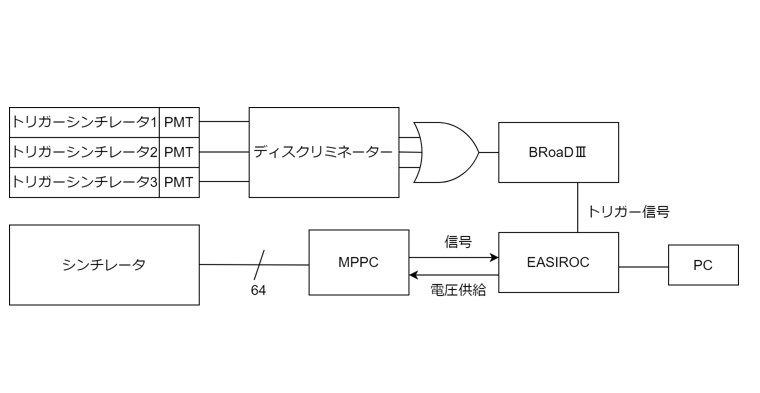
\includegraphics[height=5cm]{img/setup.jpg}
    \caption{データ取得のセットアップ}
\end{figure}
装置上部のトリガーシンチレータのいずれかに$\mu$粒子が入射したとき、データ取得が行われる。
トリガー信号はBRoaDⅢに送られ、測定に必要なPeak Hold、T Stop、Accept信号が適切な時間遅延させられてEASIROCに送られている。
Peak Holdに信号が入ると測定が開始され、T Stopに信号が入ると測定が止まり、Acceptに信号が入るまでが次の測定が始まらないインターバルの時間となっている。

\section{MPPCにおけるゲインの個体差}
MPPCの信号をEASIROCで見ると図4.9のようになる。
\begin{figure}[H]
    \centering
    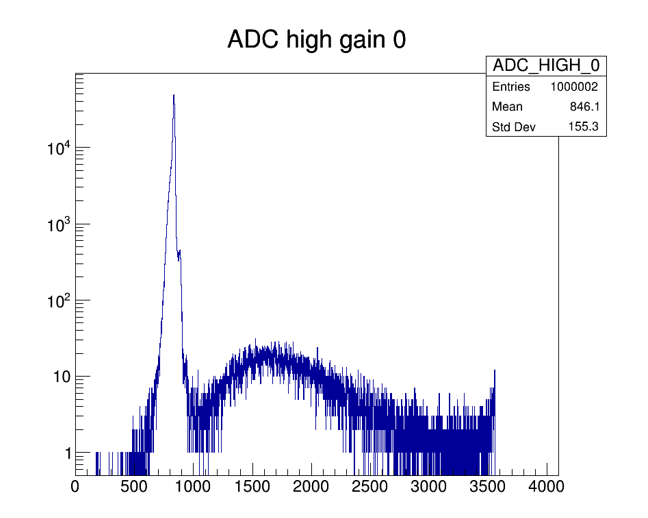
\includegraphics[height=6cm]{img/mppc_gain.jpg}
    \caption{宇宙線$\mu$粒子のMPPCにおける信号}
\end{figure}
図4.9は宇宙線$\mu$粒子が検出器に入射したときのMPPCの信号をEASIROCを用いて読み出した時のエネルギーのヒストグラムである。
$\mu$粒子が通過した際のMPPCの信号の波高分布において、波高(ADC値)はMPPCの受け取る光電子数に対応するため分布のピークから光電子数を読み取ることができる。
ADC値が850付近のピークはペデスタルである。
1番右は光電子数が多くサチュレーションしている。\\
それぞれのMPPCに同じ電圧をかけても個体差により波高が異なるので図4.9における真ん中のピークの位置も異なる。
今回の実験では粒子が通ったと判定するためのしきい値を同じくらいの値で決定するために、宇宙線$\mu$粒子を用いてキャリブレーションを行い信号のピークの位置を揃えた。
電圧を変えて3回測定し、ヒストグラムをランダウ分布でフィットしそれぞれのチャンネルのピークの位置を求めて同じ電圧をかけた時にピークの位置が同じ位置になるようにInputDACの値を調整した。
図4.10が揃える前のチャンネルごとのピークの位置で、図4.11が揃えた後の図である。
\begin{figure}[H]
    \begin{minipage}[b]{0.47\linewidth}
        \centering
        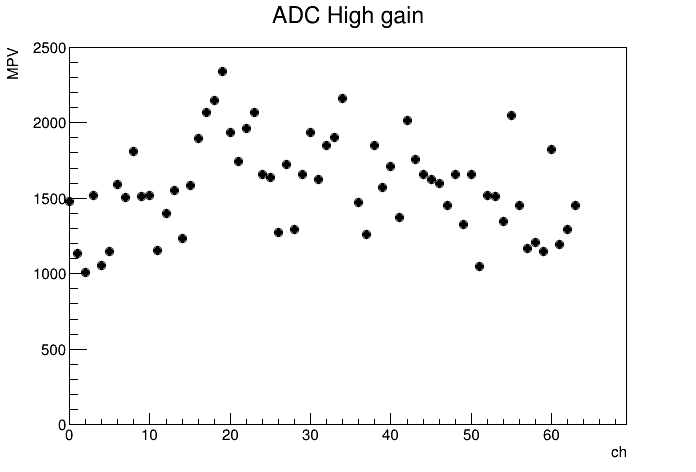
\includegraphics[height=5cm]{img/gain_before.jpg}
        \caption{ゲインを揃える前のピークのADC値}
    \end{minipage}
    \begin{minipage}[b]{0.47\linewidth}
        \centering
        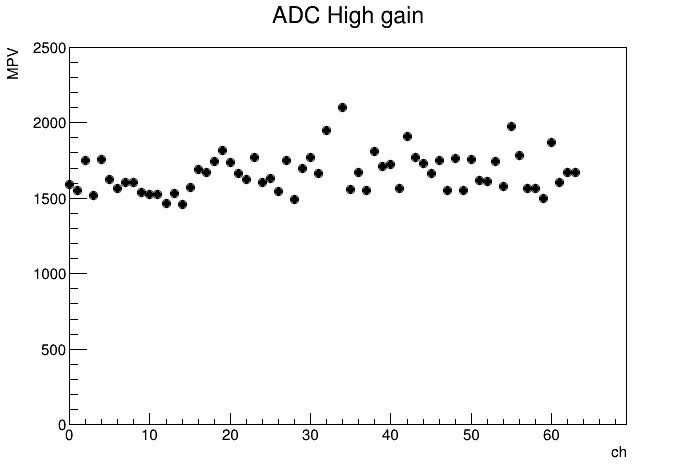
\includegraphics[height=5cm]{img/gain_after.jpg}
        \caption{ゲインを揃えた後のピークのADC値}
    \end{minipage}
\end{figure}